%==============================================================================
%  ICATC 2026 submission -- multilingual classification of bank support
%  tickets: intent, sentiment and priority, plus posterior combination.
%

%==============================================================================

\documentclass[conference,a4paper]{IEEEtran}

% IEEE requires Times. IEEEtran requests it as `ptm', which pdfLaTeX resolves
% from the standard PostScript fonts. Under a Unicode engine (XeTeX/LuaTeX) that
% request silently falls back to Latin Modern, so we load Times explicitly and
% the document then typesets in Times under every engine. newtxmath also puts
% the maths in Times, which matching the body text requires.
\usepackage[T1]{fontenc}
\usepackage{newtxtext,newtxmath}

\usepackage{cite}
\usepackage{amsmath}
\usepackage{graphicx}
\usepackage{booktabs}
\usepackage[dvipsnames]{xcolor}
\usepackage{tikz}
\usetikzlibrary{arrows.meta,positioning}
\usepackage[hidelinks]{hyperref}
\usepackage{ulem}
\newcommand\af[1]{\textbf{\textcolor{red}{AF: #1}}}
\graphicspath{{figures/}}

% Double-blind review. Keep true for the CMT review submission.
\newif\ifblind
\blindtrue

% Draft markers. Set false to measure the real page count.
\newif\ifdraftmode
\draftmodefalse
\ifdraftmode
  \newcommand{\gap}[1]{\textcolor{BrickRed}{\textbf{[GAP: #1]}}}
  \newcommand{\note}[1]{\textcolor{RoyalBlue}{\textbf{[NOTE: #1]}}}
\else
  \newcommand{\gap}[1]{}
  \newcommand{\note}[1]{}
\fi

\newcommand{\negf}{Negative-F\textsubscript{1}}
\newcommand{\macrof}{macro-F\textsubscript{1}}

\begin{document}

\title{Classification and Order Prediction of Financial\\Support Tickets Across Sinhala, Tamil,\\and Romanized Scripts}

\ifblind
  \author{\IEEEauthorblockN{Anonymous Submission}}
\else
  \author{\IEEEauthorblockN{Author One, Author Two, Author Three}
  \IEEEauthorblockA{Department, Institution\\City, Sri Lanka\\
  \texttt{author@institution.lk}}}
\fi

\maketitle

\begin{abstract}
A bank support desk must decide which waiting ticket an agent opens next, as high-severity issues such as fraud require immediate intervention under strict response windows. \af{Too many things cluttered in the opening sentence. Rephrase to clarify the problem}Published work on support ticket prioritization addresses \af{this as a classification problem which is trained with an offline dataset....and add how the rest is handled interms of}\sout{half of this operational decision by stopping at static classification and is mostly outside the banking domain}. This paper presents an operational triage and dynamic queue ordering framework that uses fine-tuned multilingual encoders to classify incoming tickets and compute dynamic urgency scores for helpdesk dispatch. Fine-tuned LaBSE encoders predict ticket intent, sentiment, and priority as continuous probability distributions, outperforming multilingual LLMs and classical baselines across English, Sinhala, Tamil, and their Romanized colloquial variants. \af{next sentence not clear...rephrase. Sentences do not start with because}Because intent accounts for 76.9\% of the uncertainty in priority, treating classification heads as independent evidence counts shared signal twice; an equal-weight log pool merges direct priority predictions with an intent-conditioned chain, reducing log loss by 27.4\% and resolving collinearity. We then specify a dynamic urgency scoring function that couples this combined posterior with elapsed waiting time, so that queue position reflects both predicted severity and accrued delay and no ticket can be starved indefinitely by construction; \af{dont add future work in abstract}its evaluation against dispatch policies under simulated load is left to future work. To train and evaluate the system, we expanded BANKING77 into a 5-track corpus of 65,385 tickets, pairing LLM-generated priority and sentiment labels, with sentiment-label quality assessed against a manually annotated gold subset.
\end{abstract}



\begin{IEEEkeywords}
multi-label classification, Sinhala, Tamil, romanized text,
transliteration, queue scheduling, multilingual NLP
\end{IEEEkeywords}

\section{Introduction}
\label{sec:intro}

A \sout{retail bank} customer support desk must decide \af{should be the next ticket to attend}which waiting ticket an agent opens next. High severity issues such as payment fraud require immediate intervention under strict response windows, \af{no need to mention in minutes}often 30 minutes or less, whereas routine balance inquiries tolerate delays of several hours. When customer requests arrive faster than staff can process them, a backlog forms. In this operating environment, the dispatch order in which tickets are assigned to agents directly determines whether service level agreements (SLAs) are upheld or violated.

Published work on customer support prioritization addresses \af{dont use words like half of the problem}only half of this operational decision by stopping at static classification. Existing methods predict static labels such as category or severity tier and evaluate performance by accuracy on held-out benchmarks. However, a set of predicted labels does not specify a dispatch order. In common practice, desks default to First Come First Served (FCFS) or group tickets by \af{add citation if it is from the paper. next part doesnt make sense}discrete argmax predictions and serve within groups by arrival order.

\af{you are talking about three probles. In the beginning say there are 3 of three problems why classification based techniques lacks.For each probelm add citations. So far i can see only one}Converting classifier outputs into an operational queue reveals challenges that static benchmarks 
hide. One is customer starvation under static triage\af{citation}. When helpdesks order tickets solely by 
static predicted categories, newly arriving urgent inquiries repeatedly overtake older requests. 
As a result, routine inquiries remain delayed in the backlog and breach service level agreements 
unless elapsed waiting time is dynamically incorporated. Second is loss of predictive uncertainty. 
Discrete argmax binning collapses a confident High priority prediction (0.99 posterior probability) 
and an uncertain 0.51 versus 0.49 near tie into the same tier, after which the queue serves them 
in arrival order. Under noisy classification, optimal scheduling requires ordering by continuous 
posterior indices rather than discrete categories \cite{argon2009priority}.


A third challenge is linguistic. In multilingual banking environments, customer messages span English, Sinhala, and Tamil, alongside informal Romanized scripts (Singlish and Tanglish). Existing public ticket datasets do not evaluate across these transliterated linguistic tracks, nor do they carry the joint priority and sentiment labels required to train an operational dispatch system.

Under this operational setting, we examine two research questions:

\textbf{RQ1} How do multilingual sentence encoders, cross-lingual masked transformers, and generative models compare across Romanized South Asian scripts under severe class imbalance? \af{not clear. is it empirically evaluate exisistng multilingual pre-trained models accuracy for .....? Dont bring class imbalance here. RQ should be specific and measureable}

\textbf{RQ2} How can a dynamic urgency score be formulated from continuous classifier probability distributions \af{dont think the waiting time is a consideration. It is external factor. Frame problem as to dynamically decide urgency based on .....what?}and elapsed waiting time to resolve inter-label dependencies and prevent queue starvation?

Our contributions are twofold. First, a \textbf{multilingual model benchmark study} spanning classical TF--IDF models, sentence encoders, masked encoders, and instruction-tuned decoders over five parallel linguistic tracks\af{what are tracks? Dataset?}. Second, an \textbf{information-theoretic posterior combination and dynamic urgency scoring framework} that merges multi-head\af{what is this?} intent, sentiment, and priority distributions via logarithmic opinion pooling \sout{(reducing log loss by 27.4\% and resolving collinearity) and} to produce a \sout{translates} continuous posteriors \af{reflecting the}\sout{into} time-dependent urgency scores.

\section{Related Work}
\label{sec:related}

\textbf{Support ticket classification and prioritization.}
Prior work frames ticket handling as single-target text classification,
including bank complaint categorization \cite{arya2026bank}. Closest to this
work, Deshmukh and Shiravale \cite{deshmukh2020priority} derive priority from
sentiment intensity and promote a complaint once it has waited past a fixed
threshold, which Section~\ref{sec:score} generalizes to a continuous accrual.
Static labels do not specify an order of service: desks default to First Come
First Served (FCFS) or to discrete priority classes, and discrete binning
discards the uncertainty continuous dispatch needs.

\textbf{Multilingual representations and transliterated scripts.}
Expanding BANKING77 \cite{casanueva2020banking77} into low-resource settings
requires representations robust to script variation: cross-lingual masked
encoders \cite{conneau2020xlmr,marone2025mmbert}, Indic-vocabulary encoders
\cite{khanuja2021muril}, sentence encoders \cite{feng2022labse}, and
instruction-tuned decoders \cite{gemmateam2025gemma3}. The Sinhala literature,
surveyed in \cite{desilva2019sinhalasurvey}, reports two patterns our benchmark
tests jointly. Architecture matters little on minority targets: adapter variants
of XLM-R move code-mixed sentiment macro-F\textsubscript{1} by only one to two
points \cite{rathnayake2022adapter}. Task-specific fine-tuning, by contrast,
dominates prompting --- on banking reviews \cite{senevirathna2025multilingual},
on native Sinhala \cite{aravinda2025sinllama}, and on Sinhala news comments
\cite{bandaranayake2025sinhala}.

\textbf{Romanized South Asian text.}
Informal romanization introduces script sensitivity and non-standard orthography
\cite{rajapakse2026script,sumanathilaka2022romanized}
that subword tokenizers handle poorly, and word-level language identification in
Latin-script Sinhala-English is context-dependent, with a CRF over character
$n$-grams beating every neural model at small data scale
\cite{smith2020codemixed}. One alternative is to reverse-transliterate into
native script before inference \cite{perera2025indonlp,sumanathilaka2026swabhasha}.
We model the romanized tracks directly, which makes our Tanglish figures a floor
rather than a ceiling.

\textbf{Annotation by prompting.}
Prompted annotation addresses label scarcity, but its errors propagate into
every downstream comparison \cite{northcutt2021labelerrors}. We therefore treat
our labels as silver and measure their ceiling against human gold.

\textbf{Dispatch under uncertainty.}
The $c\mu$ rule \cite{cox1961queues} minimizes holding cost under linear delay
penalties, while delay-dependent disciplines \cite{kleinrock1964delay} and the
accumulating priority queue \cite{stanford2014accumulating} let priority accrue
with waiting time to prevent starvation. Argon and Ziya
\cite{argon2009priority} prove that under noisy classification, ordering by a
continuous posterior index rather than a discrete argmax class minimizes
expected long-run holding cost.

\section{Multilingual Corpus and Annotation}
\label{sec:corpus}

\subsection{Multilingual Corpus Construction}

Building the system required diverse banking queries with expanded annotations. Because no public corpus provides these annotations, we construct a five-track corpus across three languages by expanding the BANKING77 dataset \cite{casanueva2020banking77}, which provides 13{,}077 English customer queries across 77 intents.

Each query was translated into four parallel tracks using Gemini 3.6 Flash \cite{geminiteam2023gemini}: native script Sinhala, native script Tamil, and informal Latin script romanizations of each (Singlish and Tanglish). Customer identifiers and class labels are aligned across all versions, producing a 5 track parallel corpus of 65{,}385 rows.

\af{Add another para as how you validated it}

\subsection{Data Cleaning and Preparation}

We dropped 55 duplicate source query pairs across all five tracks and reworded translation collisions, where two English queries were rendered identically in a target language. The corpus is partitioned into a single frozen document-level split across all five tracks: 8{,}500 training tickets (42{,}500 rows), 1{,}498 validation tickets (7{,}490 rows), and 3{,}079 test tickets (15{,}395 rows), ensuring zero query or translation leakage across splits.

\subsection{LLM Labeling and Annotation Validation}

BANKING77 provides 77 intents but not the distress and severity labels queue
prioritization needs. We generated binary sentiment (Neutral, Negative) and
three priority tiers (Low, Medium, High) with structured LLM prompts over the
English source text, copying labels across tracks. Priority was elicited
separately from intent because urgency varies within an intent: inside
\emph{transfer not received by recipient}, a general inquiry about transaction
times is Low priority whereas a time-critical request is High. Positive
sentiment was omitted because retail banking inquiries rarely express praise.

To bound label quality without leakage, 500 tickets were annotated by human
reviewers before the prompts were authored. Raw prompt output reached 0.7812
\negf{} (Cohen's $\kappa = 0.766$); the shipped labels, after a final rule
check, reach 0.7931 \negf{} (95\% confidence interval 0.667 to 0.896, agreement
0.976, $\kappa = 0.780$) against the gold annotations.

\subsection{Intent and Task Class Distributions}

\begin{figure}[!tb]
\centering
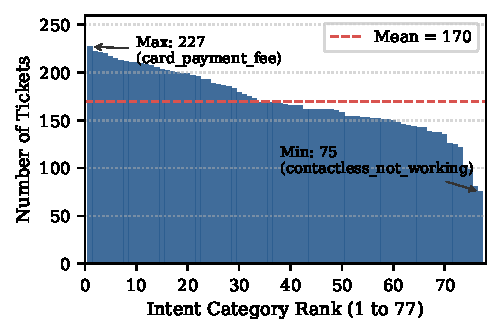
\includegraphics[width=\columnwidth]{figures/intent_distribution.pdf}
\caption{Intent distribution across all 77 categories in the BANKING77 dataset ranked by frequency ($\mu = 170$, range $75$ to $227$).}
\label{fig:intent_dist}
\end{figure}

\begin{figure}[!tb]
\centering
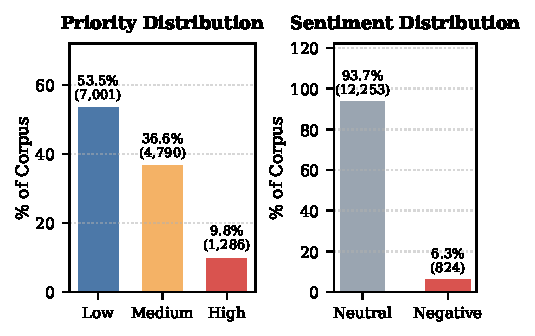
\includegraphics[width=\columnwidth]{figures/task_imbalance.pdf}
\caption{Operational class imbalance across Priority tiers (left) and Sentiment targets (right) over the 13{,}077 ticket corpus.}
\label{fig:task_imbalance}
\end{figure}

As shown in Fig.~\ref{fig:intent_dist}, BANKING77 intents display balanced coverage across all 77 categories ($\mu = 169.8$ tickets, range $75$ to $227$, normalized entropy 0.982). In contrast, the resulting operational targets exhibit severe class imbalance (Fig.~\ref{fig:task_imbalance}): Priority follows an inverse severity distribution with 53.5\% Low, 36.6\% Medium, and only 9.8\% High urgent tickets. Sentiment is 93.7\% Neutral and 6.3\% Negative, capturing customer dissatisfaction and distress for queue escalation.

\section{Multilingual Ticket Classification}
\label{sec:classifiers}

\subsection{Tokenizer Inductive Filtering}

\begin{table}[!htbp]
\caption{Tokenizer subword fertility (tokens per word) and vocabulary size.}
\label{tab:tokenizer_fertility}
\centering
\small
\setlength{\tabcolsep}{2.8pt}
\begin{tabular}{@{}lrrrrrr@{}}
\toprule
Model & Vocab & English & Sinhala & Singlish & Tamil & Tanglish \\
\midrule
LaBSE & 501k & 1.18 & 1.37 & 1.62 & 1.86 & 2.00 \\
Gemma 3 & 262k & 1.18 & 2.24 & 1.86 & 2.20 & 2.21 \\
SinLlama & 139k & 1.16 & \textbf{1.28} & 2.00 & 11.46 & 2.34 \\
Llama 3.2 & 128k & 1.16 & 7.39 & 2.00 & 11.46 & 2.34 \\
Qwen 3 & 152k & 1.16 & 5.97 & 2.02 & 9.22 & 2.35 \\
\bottomrule
\end{tabular}
\end{table}

Prior to fine-tuning, we screen candidate tokenizers for subword fragmentation across 2{,}000 sampled tickets per language track (Table~\ref{tab:tokenizer_fertility}). Parameter scale does not compensate for severe subword fragmentation: Western BPE tokenizers (Llama 3.2 and Qwen 3) shred native Indic text into 6 to 11 subwords per word, inflating sequence lengths and degrading attention efficiency. While specialized vocabulary extension in SinLlama \cite{aravinda2025sinllama} achieves high compression on native Sinhala (1.28 tokens per word), its lack of Dravidian vocabulary causes Tamil fertility to collapse to 11.46, preventing trilingual deployment. The magnitude of these penalties is consistent with survey figures of 8.83 to 12.86 subword tokens per word for Sinhala against roughly one for English \cite{desilva2019sinhalasurvey}. In contrast, Gemma 3 provides balanced fertility across all five tracks (1.18 to 2.24) with zero control character loss.

\subsection{Operational Evaluation Metrics}

Standard classification accuracy is deeply misleading under severe class imbalance. In our banking corpus, customer sentiment exhibits severe class skew with 93.7\% Neutral and only 6.3\% Negative tickets (6.33\% on the test split, 195 of 3{,}079 tickets). A naive majority class baseline predicting always Neutral achieves 93.7\% accuracy while scoring exactly 0.0000 \negf{}, failing to detect every dissatisfied customer. In our empirical class-balancing experiments, the unweighted empirical risk baseline posted the highest raw accuracy (0.9281) but the lowest \negf{} (0.3171), demonstrating that accuracy actively penalizes models that attempt to learn minority escalation signals. Consequently, we discard accuracy and adopt \negf{} as the headline evaluation metric for sentiment.

For operational priority, tickets follow an inverse severity distribution (53.5\% Low, 36.6\% Medium, and 9.8\% High). We report macro-averaged $F_1$ across all three tiers so that performance on the critical High priority escalation tier is weighted equally with the dominant Low priority class (majority class baseline scores 0.2361 \macrof{}). For intent, we evaluate 77 category macro-averaged $F_1$ across all transaction intents to ensure uniform assessment across both frequent and rare query types.

\subsection{Classical Baseline Benchmark}

\begin{table}[!htbp]
\caption{Classical TF--IDF baselines. Bal.: class-balancing arm selected on
dev (-- none, CW class weight, ROS oversampling). Best per column in bold.}
\label{tab:classical_baselines}
\centering
\scriptsize
\setlength{\tabcolsep}{2.6pt}
\begin{tabular}{@{}llrrrrrr@{}}
\toprule
Model & Bal. & English & Sinhala & Singlish & Tamil & Tanglish & Pooled \\
\midrule
\multicolumn{8}{l}{\textit{Intent (\macrof{}, 77 classes)}} \\
Linear SVM & -- & \textbf{0.9180} & \textbf{0.8666} & \textbf{0.8793} & \textbf{0.8528} & \textbf{0.6127} & \textbf{0.8308} \\
Logistic Regression & -- & 0.9096 & 0.8595 & 0.8751 & 0.8302 & 0.5854 & 0.8189 \\
SGD (mod.\ Huber) & -- & 0.9079 & 0.8489 & 0.8646 & 0.8305 & 0.5669 & 0.8115 \\
Complement NB & -- & 0.7772 & 0.6732 & 0.7194 & 0.7234 & 0.4925 & 0.6792 \\
\midrule
\multicolumn{8}{l}{\textit{Sentiment (\negf{})}} \\
Linear SVM & CW & \textbf{0.7198} & \textbf{0.6412} & \textbf{0.6633} & \textbf{0.7249} & \textbf{0.5722} & \textbf{0.6653} \\
Logistic Regression & ROS & 0.6995 & 0.6256 & 0.6545 & 0.6776 & 0.5074 & 0.6383 \\
SGD (mod.\ Huber) & ROS & 0.6842 & 0.5954 & 0.6218 & 0.6608 & 0.4577 & 0.6092 \\
Complement NB & ROS & 0.5139 & 0.5083 & 0.5302 & 0.5239 & 0.3738 & 0.4968 \\
\midrule
\multicolumn{8}{l}{\textit{Priority (\macrof{})}} \\
Linear SVM & CW & \textbf{0.9050} & \textbf{0.8848} & \textbf{0.8918} & \textbf{0.8854} & 0.7984 & \textbf{0.8734} \\
Logistic Regression & ROS & 0.8987 & 0.8810 & 0.8889 & 0.8849 & \textbf{0.7985} & 0.8706 \\
SGD (mod.\ Huber) & ROS & 0.8953 & 0.8802 & 0.8831 & 0.8853 & 0.7805 & 0.8659 \\
Complement NB & CW & 0.8643 & 0.8479 & 0.8540 & 0.8653 & 0.7782 & 0.8422 \\
\bottomrule
\end{tabular}
\end{table}

We evaluate four classical classifiers over a shared TF--IDF feature union of word 1--2 grams and character 3--5 grams, the latter carrying most of the signal on the romanized tracks, where no spelling standard exists. Linear SVM establishes the strongest classical baseline, taking the best score in 17 of the 18 task-by-track cells; Logistic Regression edges it only on Tanglish priority (0.7985 vs.\ 0.7984), and trails it by 1.2 points on pooled intent. The margin between the two linear margin based models and the SGD linear model is small, but Complement Naive Bayes falls well behind on both imbalanced targets, losing 15.2 points of pooled intent \macrof{} and 16.9 points of pooled \negf{} to the SVM, confirming that its closed-form class priors cannot substitute for discriminative training on the minority escalation classes. Tanglish is the weakest track for every model and every task, a pattern the encoder benchmark below only partly closes.

\subsection{Multilingual Encoder Benchmark}

\begin{table}[!htbp]
\caption{Multilingual encoder benchmark, per track and pooled. Best per column
within each task in bold.}
\label{tab:encoder_benchmark}
\centering
\scriptsize
\setlength{\tabcolsep}{3.2pt}
\begin{tabular}{@{}lrrrrrr@{}}
\toprule
Model & English & Sinhala & Singlish & Tamil & Tanglish & Pooled \\
\midrule
\multicolumn{7}{l}{\textit{Intent} (\macrof{}, 77 classes)} \\
Linear SVM & 0.9180 & 0.8666 & 0.8793 & 0.8528 & 0.6127 & 0.8308 \\
LaBSE      & \textbf{0.9412} & \textbf{0.9319} & \textbf{0.9034} & \textbf{0.9329} & 0.6928 & \textbf{0.8835} \\
XLM-R base & 0.9402 & 0.9244 & 0.8987 & 0.9151 & 0.7067 & 0.8801 \\
mmBERT     & 0.9374 & 0.9123 & 0.9013 & 0.9147 & 0.6566 & 0.8680 \\
MuRIL base & 0.9226 & 0.7224 & 0.8888 & 0.9080 & \textbf{0.7824} & 0.8467 \\
\midrule
\multicolumn{7}{l}{\textit{Sentiment} (\negf{})} \\
Linear SVM & 0.7198 & 0.6412 & 0.6633 & 0.7249 & 0.5722 & 0.6653 \\
LaBSE      & \textbf{0.8032} & \textbf{0.7234} & 0.6757 & \textbf{0.7606} & 0.5948 & \textbf{0.7138} \\
XLM-R base & 0.7838 & 0.7215 & 0.6361 & 0.7473 & 0.5981 & 0.7007 \\
mmBERT     & 0.7723 & 0.6766 & \textbf{0.6905} & 0.7386 & 0.6159 & 0.7000 \\
MuRIL base & 0.7967 & 0.5577 & 0.6463 & 0.7465 & \textbf{0.6235} & 0.6790 \\
\midrule
\multicolumn{7}{l}{\textit{Priority} (\macrof{})} \\
Linear SVM & 0.9050 & 0.8848 & \textbf{0.8918} & 0.8854 & 0.7984 & 0.8734 \\
LaBSE      & \textbf{0.9229} & \textbf{0.9179} & 0.8817 & \textbf{0.9130} & 0.8142 & \textbf{0.8901} \\
MuRIL base & 0.9095 & 0.8072 & 0.8861 & 0.9120 & \textbf{0.8412} & 0.8717 \\
\bottomrule
\end{tabular}
\end{table}
As shown in Table~\ref{tab:encoder_benchmark}, fine-tuned LaBSE takes the best pooled score on all three tasks among the encoders, with margins of +8.01 \af{specify units}points on both Tamil and Tanglish intent over the SVM. XLM-R base is the closest competitor, within 0.34 points pooled and 0.10 points on English intent. MuRIL trails on pooled intent (0.8467), but the pooled column conceals two facts: its deficit is concentrated in a single cell, Sinhala intent at 0.7224, where Sinhala script falls outside its vocabulary, and it takes the best Tanglish score on all three tasks, leading LaBSE by 8.96 points on Tanglish intent. XLM-R base and mmBERT were scored on priority pooled only, at 0.8872 and 0.8887. \af{add discussion for the reason}

\subsection{Generative Decoder and SLM Benchmark}

\begin{table}[!htbp]
\caption{Gemma 3 decoder benchmark. Lower panel: pooled 1B configurations;
270M was not scored on sentiment or priority. Best per column in bold.}
\label{tab:decoder_benchmark}
\centering
\scriptsize
\setlength{\tabcolsep}{3.2pt}
\begin{tabular}{@{}lrrrrrr@{}}
\toprule
Model & English & Sinhala & Singlish & Tamil & Tanglish & Pooled \\
\midrule
\multicolumn{7}{l}{\textit{Intent, per track} (\macrof{})} \\
Gemma 3 1B   & \textbf{0.9358} & \textbf{0.9221} & \textbf{0.8962} & \textbf{0.9110} & \textbf{0.6281} & \textbf{0.8635} \\
Gemma 3 270M & 0.9288 & 0.8874 & 0.8706 & 0.8907 & 0.6041 & 0.8414 \\
\bottomrule
\end{tabular}

\vspace{4pt}
\begin{tabular}{@{}lrrr@{}}
\toprule
Gemma 3 1B configuration (pooled) & Intent & Sentiment & Priority \\
\midrule
Per-task heads    & 0.8635 & \textbf{0.7126} & 0.8898 \\
One shared head   & \textbf{0.8673} & 0.7048 & \textbf{0.8904} \\
Three shared heads & 0.8616 & 0.7042 & 0.8895 \\
\bottomrule
\end{tabular}
\end{table}

We adapt Gemma 3 across 1B and 270M parameter scales using parameter-efficient LoRA  (Table~\ref{tab:decoder_benchmark}), examining three core questions:

\textbf{LoRA Projection Coverage.} Expanding LoRA coverage from attention projections alone ($q, v$) to all seven linear projections ($q, k, v, o, \mathrm{gate}, \mathrm{up}, \mathrm{down}$) produced the largest gain in the decoder study (+2.70 points on 1B, +4.56 points on 270M validation), indicating that the apparent cross-script deficit under partial LoRA was a parameter coverage artifact.

\textbf{Parameter Scaling and Minority Collapse.} The 270M model gives up 2.21 points of pooled intent \macrof{} to the 1B model (0.8414 against 0.8635), but collapses far harder on the minority target: on development data it reaches 0.5611 \negf{} against the 1B model's 0.7098, a 14.87 point gap. Compressed capacity degrades disproportionately under severe label skew.

\textbf{Joint Multi-Task Architecture.} A single Gemma 3 1B backbone equipped with a shared classification head guided by task prefix prompts achieves 0.8673 on intent, 0.7048 on sentiment, and 0.8904 on priority on the frozen test set, matching single-task encoders on priority with 0\% cross-task misrouting.

\subsection{Representation Probing Diagnostics}

To isolate representation transfer we probed frozen backbones with a linear
classifier. Pretrained LaBSE scored 0.8015 on priority and 0.7822 on intent,
substantially below the classical TF--IDF baseline (0.8734 and 0.8308), which
demonstrates that frozen representations cannot be served without supervised
fine-tuning.

\section{Information Theoretic Posterior Combination}
\label{sec:combination}

\subsection{Quantifying Inter Label Dependence}

Predicting intent, sentiment, and priority via independent output heads overlooks their joint statistical structure. Evaluating mutual information on training data ($n = 9{,}998$ tickets, in nats) reveals strong asymmetric coupling: prior entropy $H(\mathrm{prio}) = 0.9333$; $I(\mathrm{int}; \mathrm{prio}) = 0.7178$ (resolving 76.9\% of priority entropy); $I(\mathrm{sent}; \mathrm{prio}) = 0.0172$ (1.8\%); and $I(\mathrm{sent}; \mathrm{prio}\mid \mathrm{int}) = 0.0149$ (86.6\% survives conditioning). Thus, intent provides a dominant, overlapping signal for priority, while sentiment acts as a sparse, non-redundant orthogonal adjustment. Fitting linear mixtures of the form $w_P P(\mathrm{prio}) + w_I P(\mathrm{int})$ induces collinearity, as weights sum redundant estimates of the same underlying event.

\subsection{Candidate Combination Rules and Evaluation}

We benchmark five probabilistic combination mechanisms on the frozen test split: (i)~\emph{Marginal}: direct priority head $P_{\mathrm{head}}(\mathrm{prio}\mid x)$; (ii)~\emph{Stacked Generalization}: a multinomial logistic meta learner \cite{wolpert1992stacked}; (iii)~\emph{Intent Chain}: a classifier chain \cite{dembczynski2010pcc} marginalizing over intent, $P_{\mathrm{chain}}(k\mid x) = \sum_{i=1}^{77} P(\mathrm{int}{=}i\mid x)\, P(\mathrm{prio}{=}k\mid \mathrm{int}{=}i)$, where contingency $P(\mathrm{prio}\mid \mathrm{int})$ is estimated on training gold labels; (iv)~\emph{Full Chain}: conditioning priority jointly on intent and sentiment; and (v)~\emph{Log Pool}: the normalized geometric mean of the direct priority head and the intent chain:
\begin{equation}
P_{\mathrm{pool}}(k\mid x) \propto \bigl(P_{\mathrm{head}}(\mathrm{prio}{=}k\mid x)\, P_{\mathrm{chain}}(k\mid x)\bigr)^{1/2}
\label{eq:logpool}
\end{equation}
Logarithmic opinion pooling aggregates dependent experts sharing background information without linear double counting.

\begin{table}[!tb]
\caption{Priority combination rules on the frozen test split.}
\label{tab:combination}
\centering
\footnotesize
\setlength{\tabcolsep}{4pt}
\begin{tabular}{@{}lrr@{}}
\toprule
Combination Rule & Log Loss & \macrof{} \\
\midrule
Marginal (priority head alone)    & 0.3697 & 0.8901 \\
Stacked generalization \cite{wolpert1992stacked} & 0.3333 & 0.8914 \\
Intent chain \cite{dembczynski2010pcc} & 0.3160 & 0.8742 \\
Full chain (intent + sentiment)   & 0.3111 & 0.8749 \\
\textbf{Log pool (head $\times$ intent chain)} & \textbf{0.2683} & \textbf{0.8983} \\
\bottomrule
\end{tabular}
\end{table}

Selection is governed by multiclass log loss (cross entropy) to ensure calibrated continuous posteriors for downstream queue scheduling (Table~\ref{tab:combination}). Equal weight log pooling attains the lowest log loss (0.2683) and highest \macrof{} (0.8983), reducing log loss by 27.4\% over the standalone priority head (0.3697) and effectively resolving label collinearity.

\subsection{The Calibration Trap in Operational Ordering}

On development data, fine-tuned LaBSE exhibits an Expected Calibration Error (ECE) of 0.0658. Post hoc temperature scaling \cite{guo2017calibration} reduces ECE to 0.0192. However, examining temperature scaled posteriors for operational ranking reveals a critical trade off: temperature scaling pulls logits toward uniform entropy, compressing the dynamic range that differentiates urgent incidents from routine inquiries. While post hoc calibration optimizes population level probability reliability, it diminishes score separation across distinct priority tiers. Because dispatch ordering relies on ranking separation rather than population level marginal calibration, we emit uncalibrated pooled posteriors.

\section{Dynamic Urgency Scoring and Dispatch}
\label{sec:score}

\subsection{Formulation of the Ticket Urgency Score}

The dynamic queue ordering mechanism translates continuous posteriors and elapsed waiting time into an operational priority scalar. For waiting ticket $t$ evaluated at dispatch time $\tau$, the Ticket Urgency Score $U(t, \tau)$ couples intrinsic severity $S(t)$ with multiplicative aging:
\begin{align}
U(t,\tau) &= S(t)\,\bigl(1 + \alpha\, a(t,\tau)\bigr), \quad a(t,\tau) = \frac{\tau - \mathrm{arrival}(t)}{D_k} \label{eq:tus}\\
S(t) &= w_P\,\hat{\mathbb{E}}[\mathrm{sev}\mid t] + w_S\,\hat{P}(\mathrm{Neg}\mid t) + w_I\,\kappa(\hat{\imath}(t)) \label{eq:severity}
\end{align}
subject to simplex weights $w_P, w_S, w_I \ge 0$, $\sum_j w_j = 1$, aging coefficient $\alpha \ge 0$, and class response deadline $D_k$.

Equation~\eqref{eq:tus} integrates three principles:
(i)~\textbf{Continuous Expected Severity}: Rather than discrete argmax assignment, expected severity $\hat{\mathbb{E}}[\mathrm{sev}\mid t] = \sum_k \hat{p}_k(t)\,\mathrm{sev}_k$ over $\mathrm{sev} = (0, 0.5, 1.0)$ smoothly separates confident Low tickets ($S \approx 0$) from borderline 0.51/0.49 ties ($S \approx 0.25$), preventing premature dispatch of uncertain items.
(ii)~\textbf{Empirical Intent Criticality Prior}: The prior $\kappa(i) = \hat{P}(\mathrm{High}\mid \mathrm{int}=i)$ measures historical escalation risk on training data. Critical intents (e.g., lost or compromised card, where $\kappa \approx 1.0$) guarantee high urgency even when customer wording appears calm.
(iii)~\textbf{Multiplicative Relative Aging}: Normalizing wait time by class SLA $D_k \in \{30, 120, 480\}$ minutes ensures aging scales with intrinsic severity. Long waiting Low tickets accelerate as $a(t, \tau) \to 1$, eventually overtaking fresh Medium inquiries to structurally eliminate starvation. A discrete form of this idea appears in \cite{deshmukh2020priority}, where a citizen complaint waiting past a fixed threshold is promoted one tier; Eq.~\eqref{eq:tus} replaces that single step with a continuous accrual normalized by the class deadline.

\subsection{Parameter Fitting and Signal Ablation}

Grid search on the development set over the 3 simplex (0.05 resolution) and exponential $\alpha$ yields optimal weights $w = (0.80, 0.10, 0.10)$ and $\alpha = 16$. The optimization landscape is stable: 71 of 231 simplex points lie within 5\% of optimal holding cost across $w_P \in [0.10, 0.90]$, reflecting the strong informational overlap between intent and priority identified in Section~\ref{sec:combination}. Component ablation on development gold sets confirms that grounding priority in the empirical intent prior $\kappa(i)$ shields critical accounts from false-negative omissions, while the sentiment adjustment $w_S$ selectively elevates frustrated customers within their priority tier without destabilizing overall queue ordering.

\section{Limitations}
\label{sec:limitations}

Every reported score measures agreement with LLM generated silver labels whose accuracy against human judgment is bounded by our 500 ticket gold validation ceiling (0.7931 \negf{}, $\kappa = 0.780$), while priority tiers carry unadjudicated silver noise in the rare High class (9.8\%). Labeling 
prompts were authored and evaluated solely on English source text and copied identically across tracks, 
overlooking language specific nuances in how urgency and grievance are expressed natively. The corpus expands from English BANKING77 via automated translation pipelines; translated queries inherit Western banking concepts (such as virtual card provisioning) that diverge from South Asian retail payment ecosystems, and cannot fully replicate the organic code-mixing, colloquial idioms, and non-standard phonetic spelling native to Sinhala, Tamil, Singlish, and Tanglish customer chat. All models were tuned on development data and opened the frozen test partition once as benchmark comparisons rather than field generalization guarantees. The prior evidence we build on is also thicker for Sinhala than for Tamil: we found no Tamil-English word-level code-mixed study of comparable rigour to \cite{smith2020codemixed}, so the Tamil and Tanglish tracks are less well grounded in prior work than their Sinhala counterparts, and the 312$\times$ romanization penalty reported in \cite{rajapakse2026script} is intrinsic perplexity on decoder-only models rather than encoder classification accuracy, so it motivates rather than predicts the gaps we measure. Finally, post hoc temperature scaling optimizes ECE by compressing logit variance, demonstrating that conventional probability calibration trades off directly against score separation in operational dispatch.

\section{Conclusion}
\label{sec:conclusion}

This paper contributed a five-track multilingual support ticket corpus carrying
intent, sentiment, and priority labels, a cross-script benchmark of four model
families on all three targets, and a measurement of the statistical dependence
between the targets.

Fine-tuned LaBSE gives the best pooled intent \macrof{} (0.8835 against 0.8308
for the strongest classical baseline), a margin significant under both paired
bootstrap and McNemar tests. On sentiment and priority the four encoders, the
three Gemma 3 1B configurations and the classical SVM fall inside one another's
intervals --- pooled \negf{} spans 0.679 to 0.714 and pooled priority 0.872 to
0.890, with the best priority score belonging to a decoder. So we claim no
architectural advantage on those targets. The dominant source of variation is
script rather than architecture: romanized Tanglish costs every model 14 to 32
points of intent \macrof{} relative to English, and MuRIL, which ranks last on
pooled intent, has both the smallest romanization gap and the best absolute
Tanglish score on all three tasks. Measuring inter-label mutual information
showed that intent explains 76.9\% of priority entropy, and an equal-weight
logarithmic pool of the direct priority head and an intent-conditioned chain
cuts log loss by 27.4\% where a linear mixture of the same estimates is
collinear by construction.

Every score is bounded by a measured rather than assumed annotation ceiling
(0.7931 \negf{} at $\kappa = 0.780$ against human gold). The urgency score of
Section~\ref{sec:score} is specified, not validated: measuring it against
established dispatch policies under load, and closing the romanization gap, are
the natural next steps.


%==============================================================================
%  Acknowledgment
%
%  IEEEtran.cls (v1.8b) provides no acknowledgment command or environment --
%  the section is author-supplied \section*{} prose and is optional. IEEE uses
%  the SINGULAR "Acknowledgment" for regular papers; the plural form is
%  Computer Society style, selected by the `compsoc' class option, which this
%  paper does not use.
%
%  Compiled in both the blinded and camera-ready builds: the text names no
%  individual, institution, grant, or project, so it carries no identifying
%  information and is safe under double-blind review.
%==============================================================================

\section*{Acknowledgment}
In accordance with the conference policy on AI-generated
text, Parts of this manuscript were drafted with a large language
model (Claude Opus 5) from author-
supplied results, outlines, and notes. Google Gemini (3.6
Flash) was used to produce the non-English corpus renderings
and the sentiment and priority labels described in Section IV;
this use forms part of the reported methodology rather than the
manuscript writing. No AI system generated the experimental
results, numerical values, or tables. The authors reviewed the
AI-assisted material and take responsibility for the accuracy
and integrity of the manuscript.

\bibliographystyle{IEEEtran}
\bibliography{refs}

\end{document}
